\chapter{Procedure}
\section{Equipment}
The necessary equipment for this lab is as follows:
\begin{itemize}
  \item 2 meter aluminum rod
  \item Table clamp
  \item Swivel clamp or $90^\circ$ Offset Clamp
  \item Meter Stick
  \item $\frac{1}{2}"$ and $\frac{3}{8}"$ steel ball
  \item Freefall Adapter - PASCO \#ME
  \item PASCO 750 Interface box
  \item PASCO Interface box power cord and SCSI Interface Card
  \item Laptop Computer w/ Data Studio
\end{itemize}

\section{Procedure}

\section{A. Apparatus Setup}
Setup the apparatus as shown in the picture below. Make sure that the clamps are tight,
but not over tight. The clamp holding the apparatus should be tight enough to not allow
the apparatus to move around. Makre sure that the small thumb screw on the ball
clamp is on top.

\begin{figure}[htbp]
  \centerline{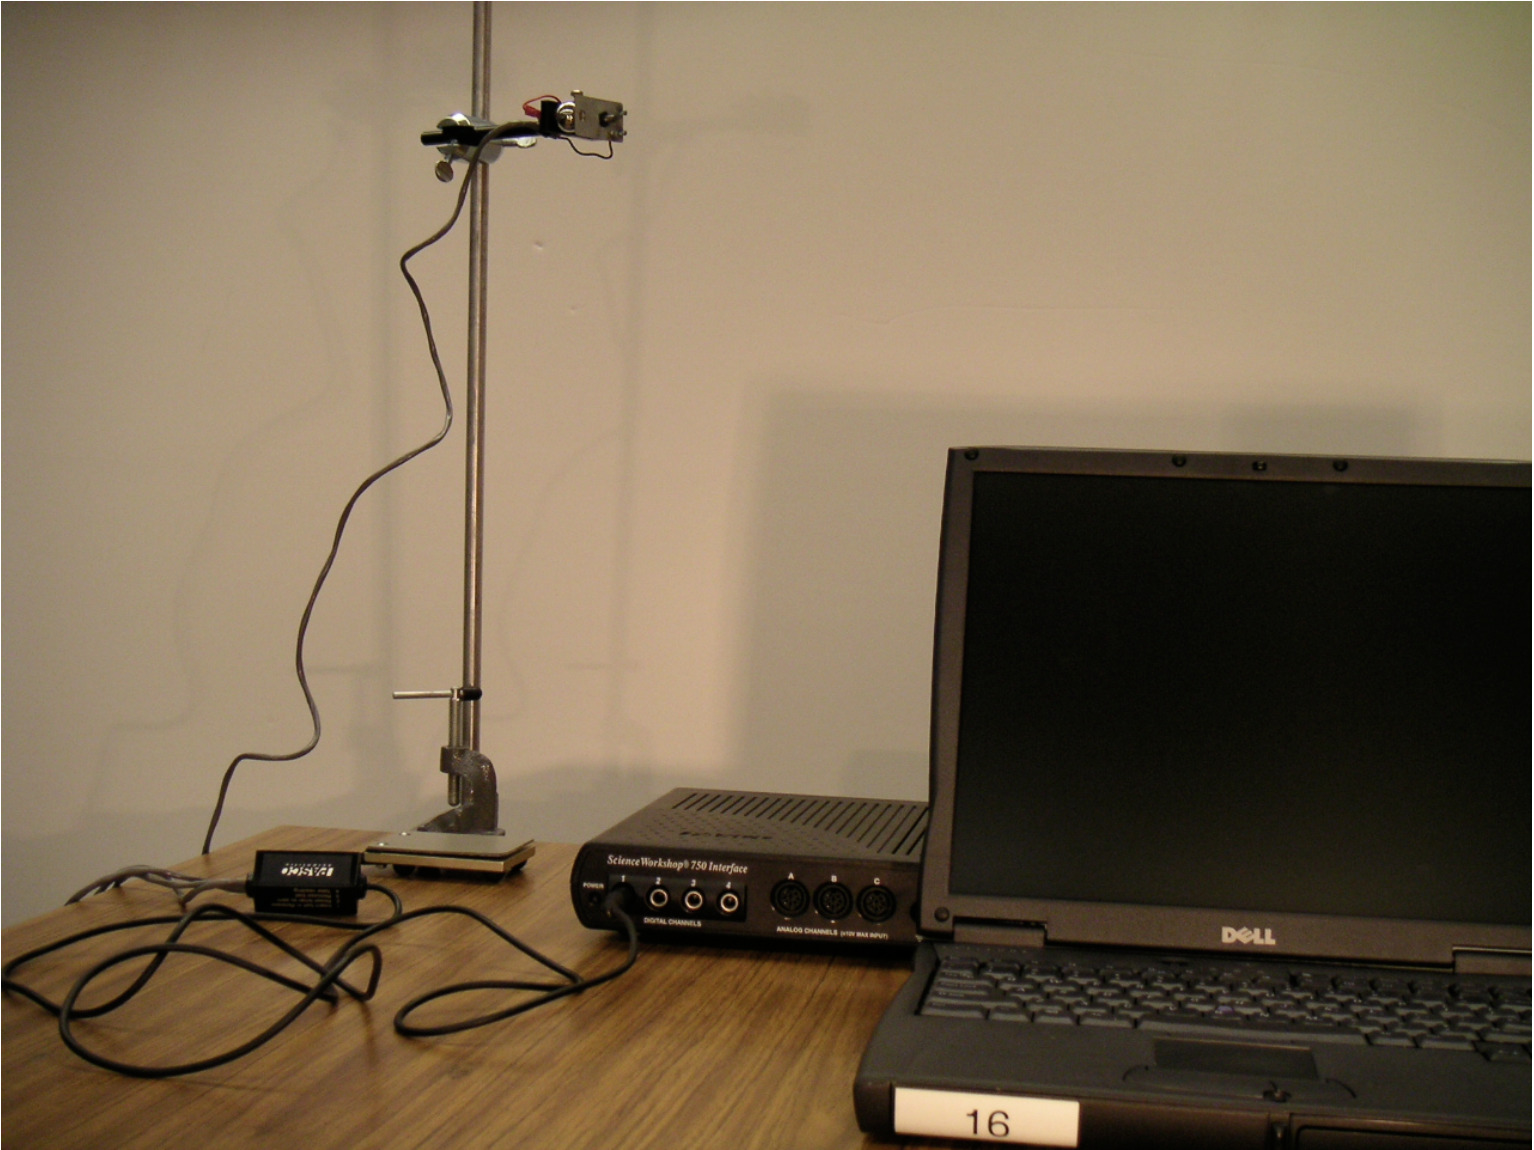
\includegraphics{resources/photo1.jpg}}
\end{figure}
